

\documentclass{article}
\usepackage{times}
\usepackage{german}
\usepackage{fancyhdr}
\usepackage[utf8]{inputenc}
\usepackage{graphicx}

\title{Datenstrukturen\\Praxiseinheit 3}
\author
{
	Sascha Ebert\\
	MatNr: 177182\\
	\texttt{sascha.ebert@s2006.tu-chemnitz.de}\\
	\texttt{https://github.com/Sighter/Datenstrukturen-p03}\\
}

\date{\today}

\begin{document}
\maketitle

\begin{abstract}
Anbei finden sie Erläuterungen zu den Aufgaben der 3. Praxiseinheit.
Alle anderen Programmcode-bezogenen Aufgaben finden sie im Quelltext an den jeweiligen Positionen
erläutert. Es somit auch möglich das oben vermerkte Git-Repository zu nutzen um den Quelltext
zu betrachten. Die aufgabenbezogenen Kommentare sind mit `Exercise' oder `Hint' gekennzeichnet.
\end{abstract}

\section*{Aufgabenzuordnung}
\begin{tabular}{ c l l }
  Aufgabe & Datei & Funktion/Methode\\
  \hline
  Datenstruktur & intList.h & struct intElem\\
  a - c  & network.cpp & network::find\_node\\
  Beispielliste  & main.cpp & main
\end{tabular}

\section*{Anmerkungen}
Alle Rufe auf externe libraries wurden mit der Preprozessor-Anweisung ''\#ifdef VERBOSE'' geklammert.
Sie können also mit der Anweisung ''\#define VERBOSE'' die printf-Funktionalität wieder herstellen.

\newpage
\section*{Beispielliste}
\includegraphics[width=12cm]{structure}

Hier zu sehen ist die Beispielliste nachdem alle Werte entfernt wurden, welche durch 2, 3, und 5 Teilbar sind.
Der Speicher ist dadurch zunehmend fragmentiert.

\end{document}


